%!TEX root = Slic3r-Manual.tex

\subsection{\texttt{Post-Processing Scripts}} % (fold)
\label{sec:post_processing_scripts}
\index{scripts}
\index{post processing}

There may be times when the G-Code generated by Slic3r has to be tweaked or modified after it has been created.  For this reason there exists the ability to run arbitrary scripts as part of the final steps in the slicing process\footnote{\texttt{https://github.com/alexrj/Slic3r/wiki/Writing-post-processing-scripts}}.

\index{Print Settings!Output options!Post-processing scripts}
In the \texttt{Output options} subsection of the \texttt{Print Settings} tab lies the \texttt{Post-processing scripts} option.  The absolute path to each script can be added, separated by semicolons. Each scripts should be recognised by the host system, and be executable.

\begin{figure}[H]
\centering
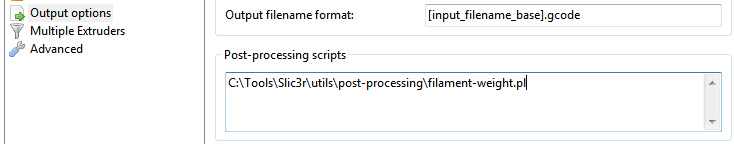
\includegraphics[keepaspectratio=true,width=1\textwidth]{advanced/post_processing_scripts/post_processing_scripts_options.png}
\caption{Post-processing script option.}
\label{fig:post_processing_scripts_options}
\end{figure}

Each script will be passed the absolute path of the G-Code file that Slic3r generates.  All Slic3r configuration options are made available to the scripts by way of environment variables.  These all begin with \texttt{SLIC3R\_}.  The following script would write out all Slic3r options to standard output:

\begin{figure}[H]
\small
\begin{verbatim}
        #!/bin/sh
        echo "Post-processing G-code file: $*"
        env | grep ^SLIC3R
\end{verbatim}
\caption{Example post-processing script to display Slic3r environment variables.}
\label{fig:exaple_post_processing_script_env_vars}
\end{figure}

Example scripts can be found in the GitHub repository\footnote{\texttt{https://github.com/alexrj/Slic3r/tree/master/utils/post-processing}}.


Perl's in-place mode (\texttt{perl -i}) makes it easy to modify the contents of the G-Code file, without having to copy, edit, then replace the original.  The following example will simply output the contents to standard output:

\begin{figure}[H]
\small
\begin{verbatim}
        #!/usr/bin/perl -i
        use strict;
        use warnings;

        while (<>) {
             # modify $_ here before printing
             print;
        }
\end{verbatim}
\caption{Example post-processing script to print each line to output.}
\label{fig:exaple_post_processing_script_print_lines}
\end{figure}

% subsection post_processing_scripts (end)
